\subsection{INVERSE CIRCULAR FUNCTIONS}

The restriction of the function \(\sin x\) to the interval \([- \pi/2, +\pi/2]\) is strictly increasing; one denotes its inverse by \(\operatorname{Arc}\sin x\) , which is thus a strictly increasing continuous map of the interval \([-1, +1]\) onto \([- \pi/2, +\pi/2]\) (fig.~6). The formula for differentiating inverse functions (I, p.~9, prop. 6) gives the derivative of this function

\[
\mathrm{D} (\operatorname{Arc} \sin x) = \frac {1}{\cos (\operatorname{Arc} \sin x)}.
\]

Since \(-\pi/2 \leqslant \operatorname{Arc} \sin x \leqslant \pi/2\) we have \(\cos(\operatorname{Arc} \sin x) \geqslant 0\) , and since

\[
\sin (\operatorname{Arc} \sin x) = x,
\]

we have \(\cos(\operatorname{Arc}\sin x)=\sqrt{1-x^{2}}\) , from which

\[
\mathrm{D} (\operatorname{Arc} \sin x) = \frac {1}{\sqrt {1 - x ^ {2}}}.\tag{16}
\]

Likewise the restriction of \(\cos x\) to the interval \([0, \pi]\) is strictly decreasing; one denotes its inverse function by \(\operatorname{Arc}\cos x\) , and this a strictly decreasing map of \([-1, +1]\) onto \([0, \pi]\) (fig.~6). Moreover

\pandocbounded{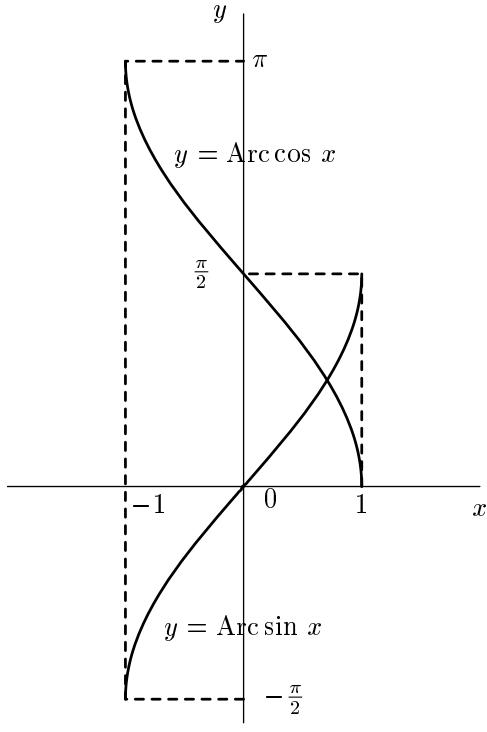
\includegraphics[keepaspectratio]{images/part001_f987f09f.jpg}}\\
Fig. 6

\[
\sin \left(\frac {\pi}{2} - \operatorname{Arc} \cos x\right) = \cos (\operatorname{Arc} \cos x) = x
\]

and since \(-\pi / 2 \leqslant \pi / 2 - \operatorname{Arc} \cos x \leqslant \pi / 2\) , we have

\[
\operatorname{Arc} \cos x = \frac {\pi}{2} - \operatorname{Arc} \sin x\tag{17}
\]

from which in particular it follows that

\[
\mathrm{D} \big (\operatorname{Arc} \cos x \big) = - \frac {1}{\sqrt {1 - x ^ {2}}}.\tag{18}
\]

Finally, the restriction of \(\tan x\) to the interval \(]-\pi/2, +\pi/2[\) is strictly increasing; one denotes its inverse by Arc \(\tan x\) , and this is a strictly increasing map from R onto \(]-\pi/2, +\pi/2[\) (fig.~7); we have

\[
\lim _ {x \rightarrow - \infty} \operatorname{Arc} \tan x = - \frac {\pi}{2}, \quad \lim _ {x \rightarrow + \infty} \operatorname{Arc} \tan x = \frac {\pi}{2},
\]

and, by applying the formula for differentiating inverse functions and formula (15) of III, p.~95, we have

\[
\mathrm{D} \big (\operatorname{Arc} \tan x \big) = \frac {1}{1 + x ^ {2}}.\tag{19}
\]

\pandocbounded{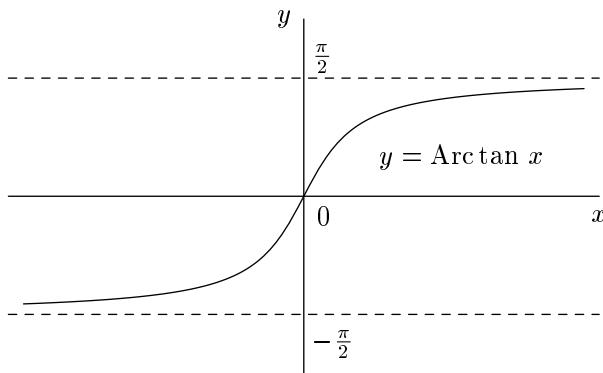
\includegraphics[keepaspectratio]{images/part001_f81b3ea6.jpg}}\\
Fig. 7

